\section{Задание 5}

Адрес команды \#!: 80000018

\begin{figure}[ht!]
\centering
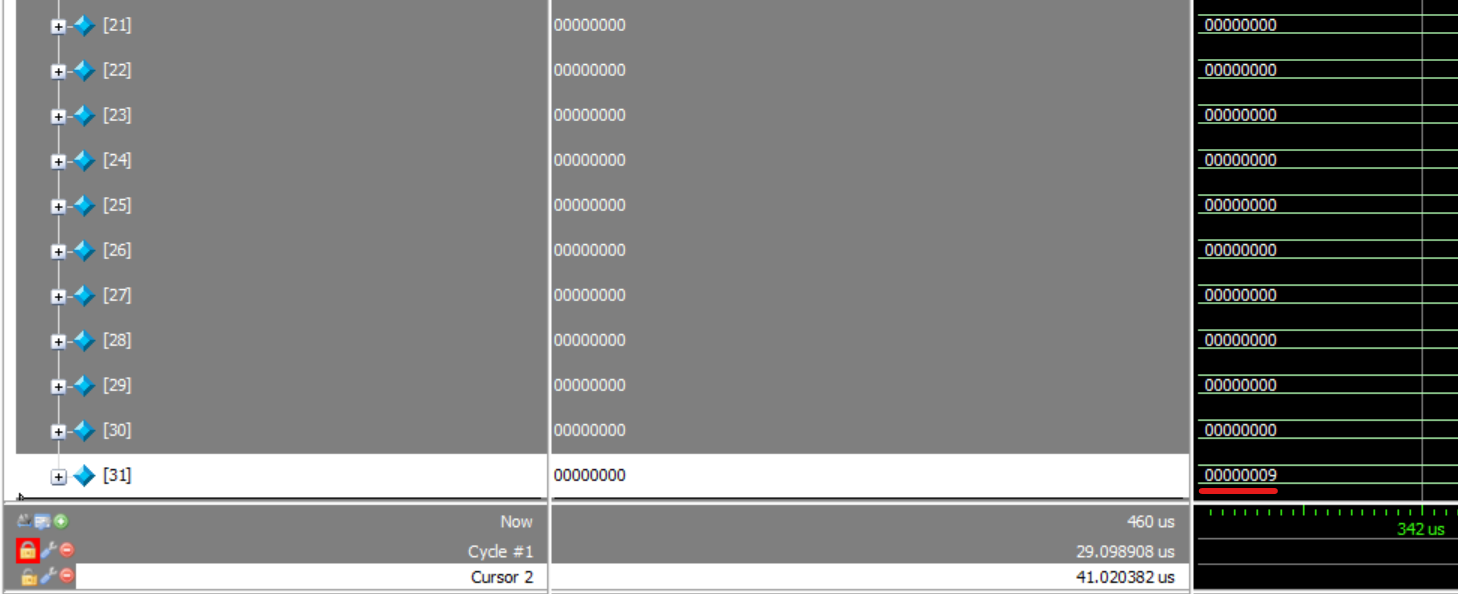
\includegraphics[width=170mm]{./img/task5.png}
\caption{Результат в регистре x31 \label{overflow}}
\end{figure}

\begin{figure}[ht!]
\centering
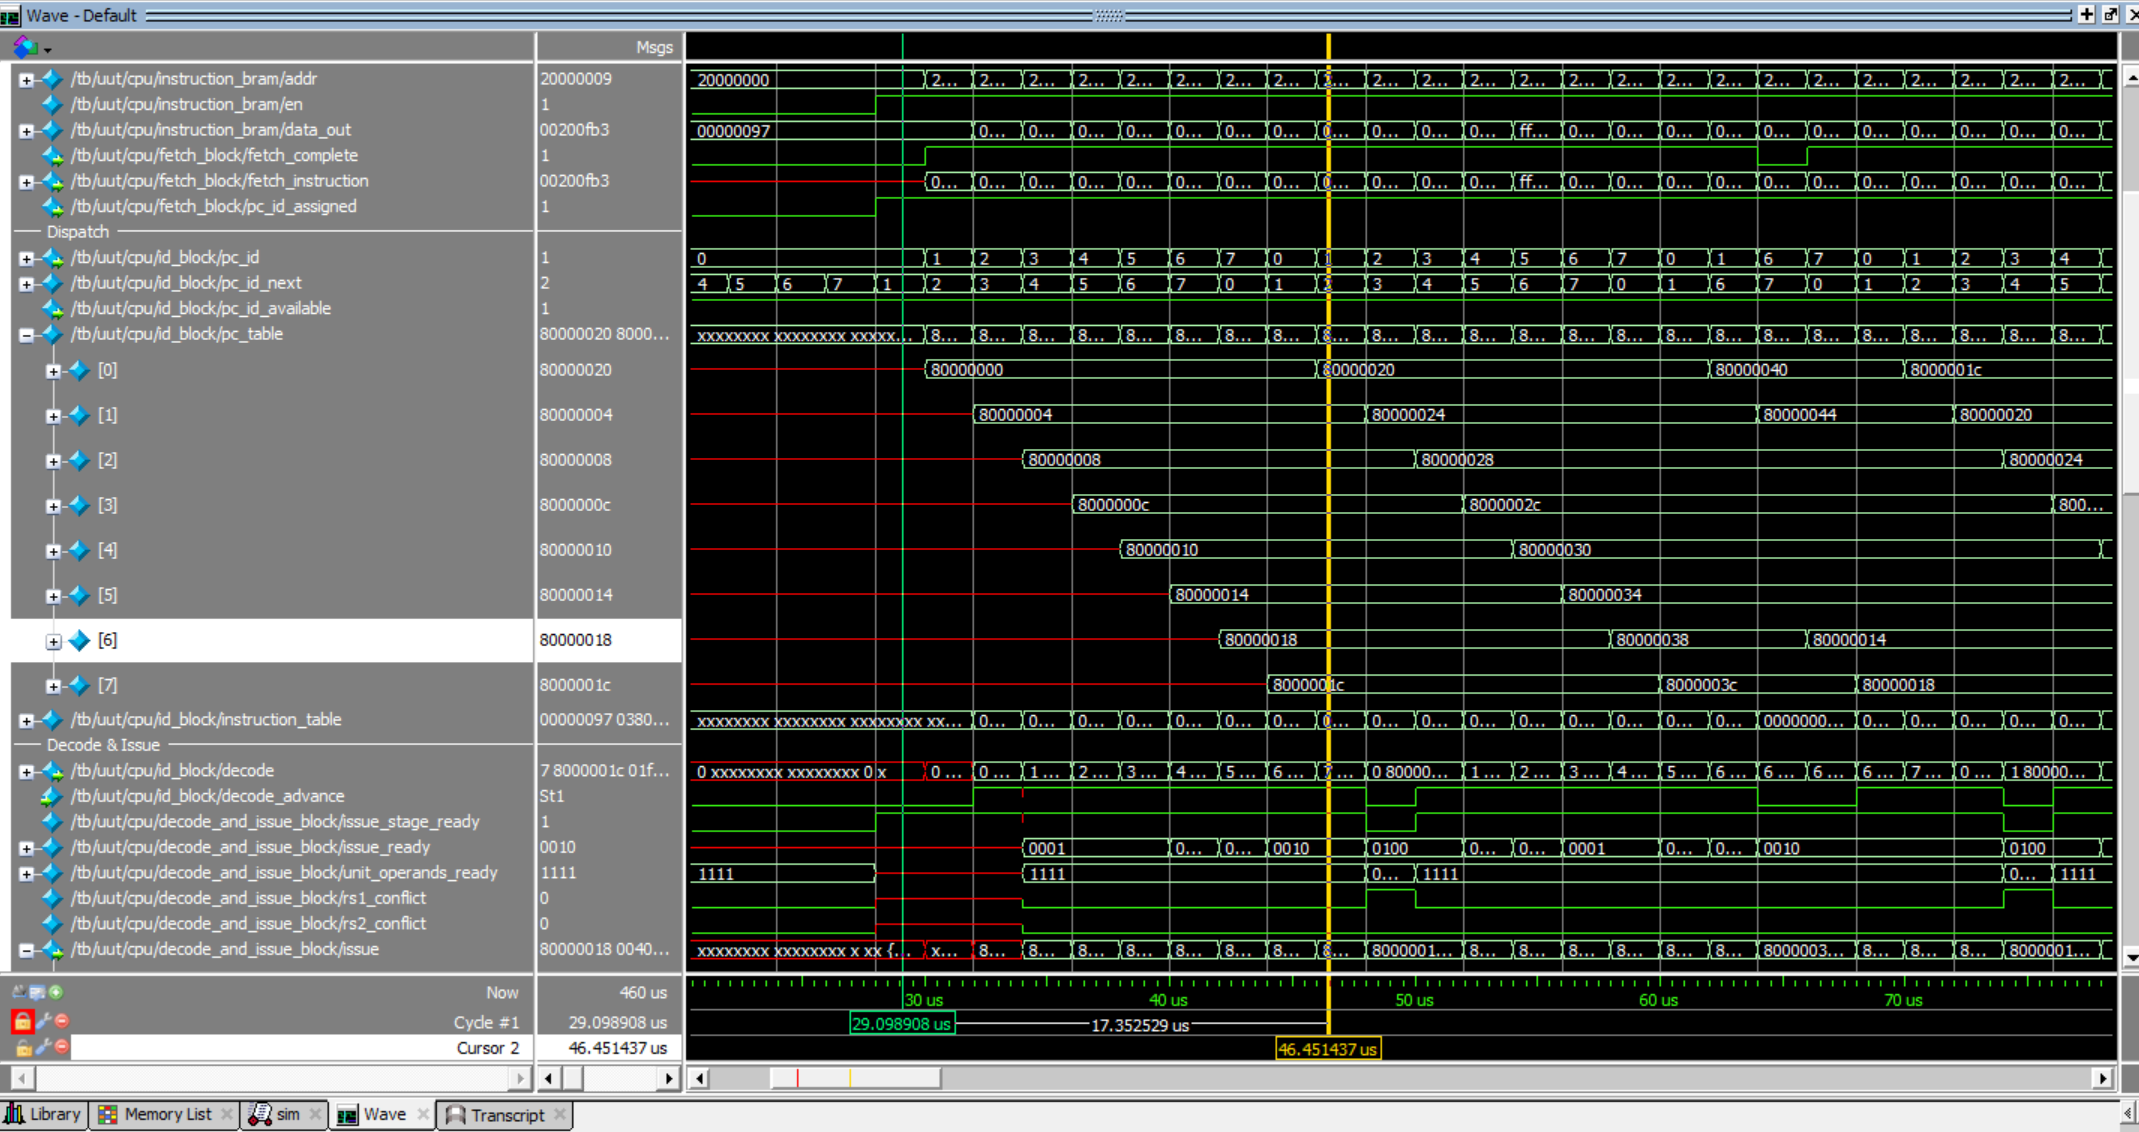
\includegraphics[width=170mm]{./img/task5_1.png}
\caption{Выборка и диспетчерезация \label{overflow}}
\end{figure}

\begin{figure}[ht!]
\centering
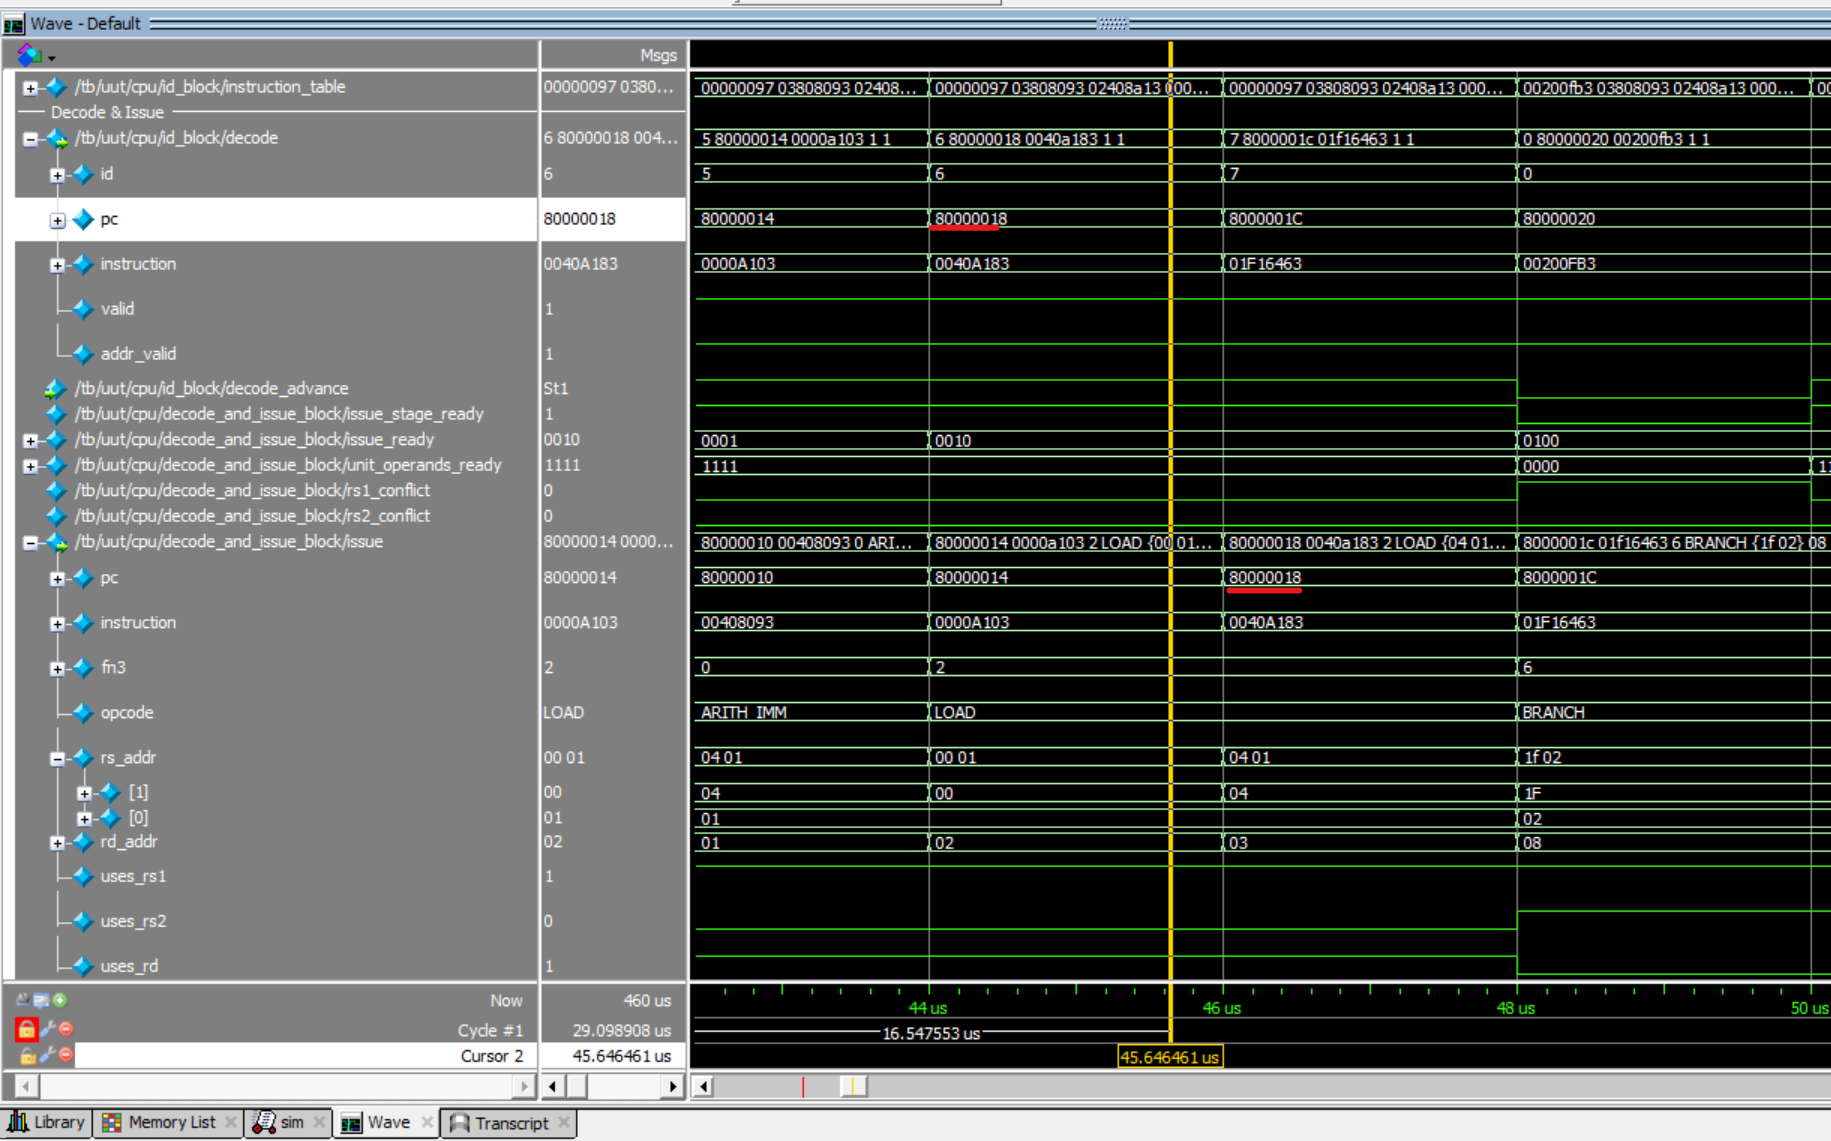
\includegraphics[width=170mm]{./img/task5_2.png}
\caption{Декодирование и планирование \label{overflow}}
\end{figure}

\begin{figure}[ht!]
\centering
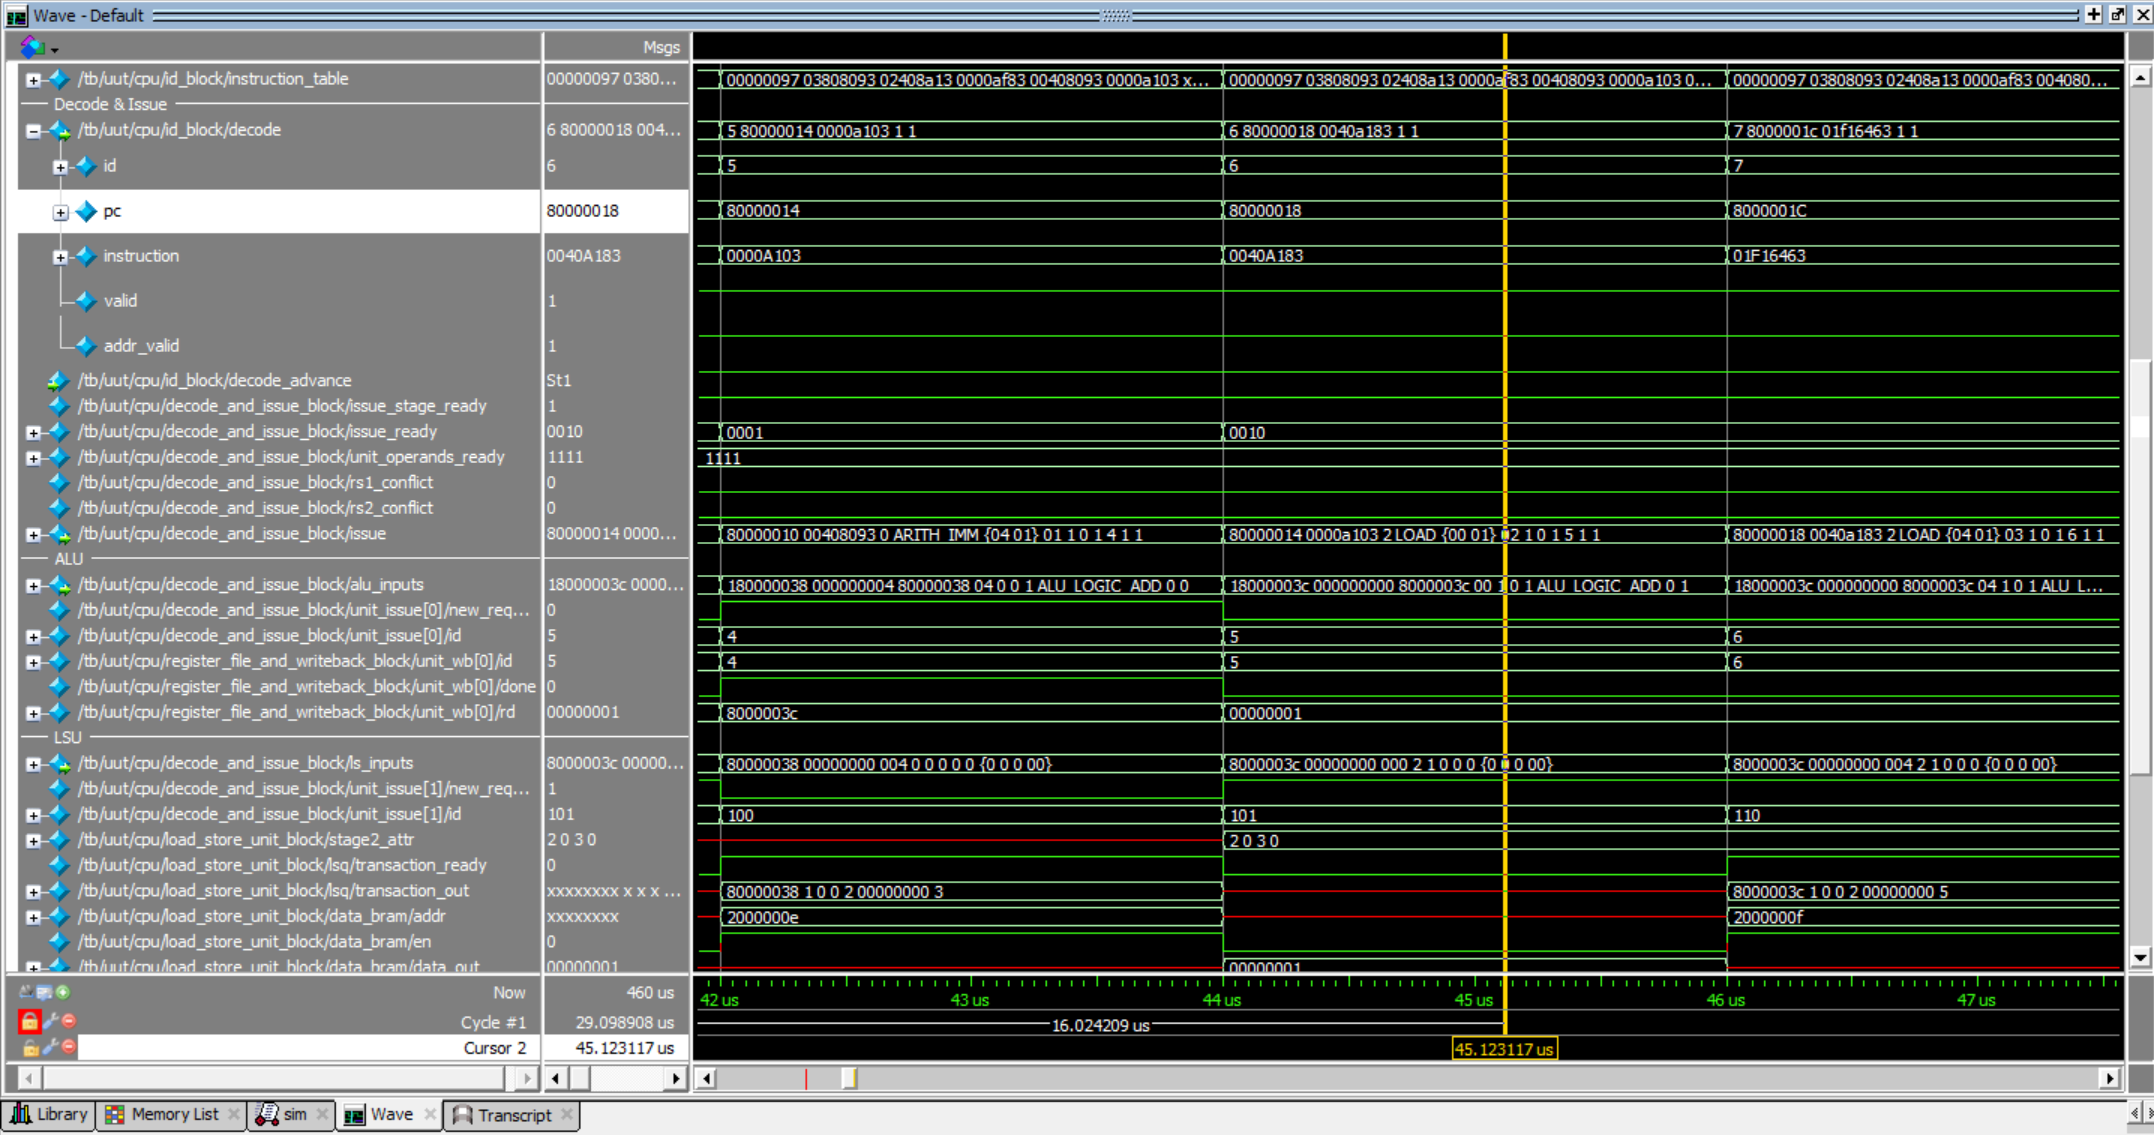
\includegraphics[width=170mm]{./img/task5_3.png}
\caption{Выполнение \label{overflow}}
\end{figure}

\clearpage

\begin{figure}[ht!]
    \centering
    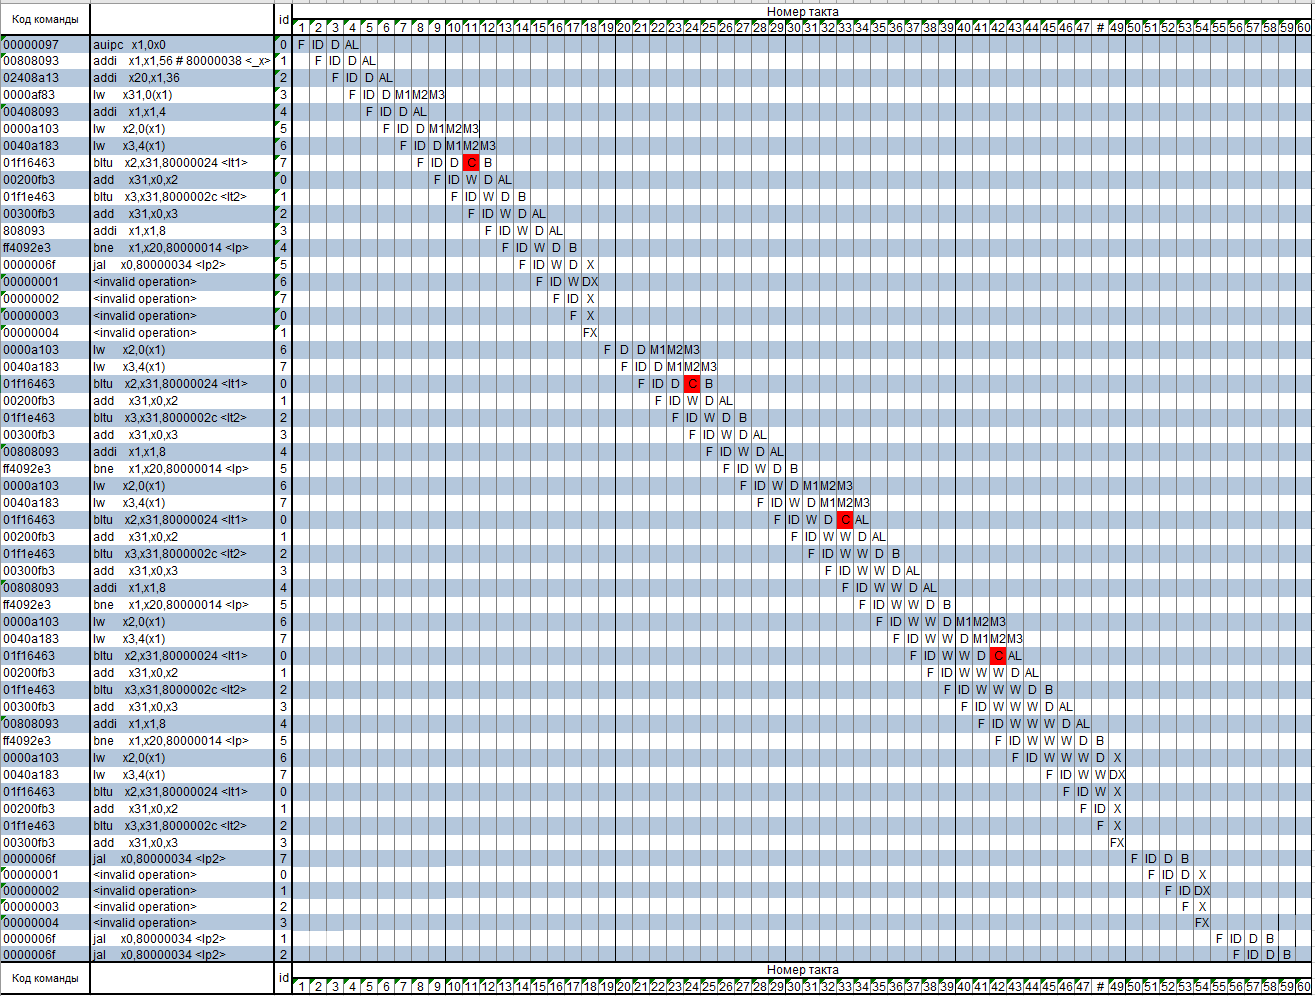
\includegraphics[width=170mm]{./img/trasa.png}
    \caption{Трасса работы программы\label{overflow}}
\end{figure}

Конфликты возникают из-за того, что мы обращаемся к значению в регистре, до того как оно было еще записано.
Оптимизировать программу можно тем, что сначала загрузить одно значение, затем увеличить указатель, затем то 
же само сделать и для второго числа, и только после этого работать с регистрами.

\clearpage

Оптимизированная программа:
\begin{lstlisting}
    .section .text
    .globl _start;
    len = 9 #Размер массива
    enroll = 2 #Количество обрабатываемых элементов за одну итерацию
    elem_sz = 4 #Размер одного элемента массива

_start:
    la x1, _x
    addi x20, x1, elem_sz*len #Адрес элемента, следующего за последним
    lw x31, 0(x1)
    addi x1, x1, elem_sz*1
lp:
    lw x2, 0(x1)
    addi x1, x1, elem_sz
    lw x3, 0(x1) #!
    addi x1, x1, elem_sz
    bltu x2, x31, lt1
    add x31, x0, x2
lt1:    bltu x3, x31, lt2
    add x31, x0, x3 
lt2:
    bne x1, x20, lp
lp2: j lp2

    .section .data
_x: .4byte 0x1
    .4byte 0x2
    .4byte 0x3
    .4byte 0x4
    .4byte 0x5
    .4byte 0x6
    .4byte 0x7
    .4byte 0x8
    .4byte 0x9
    
\end{lstlisting}

\clearpage

Дизассемблированный код:
\begin{lstlisting}{}
    Disassembly of section .text:
    
    80000000 <_start>:
    80000000:       00000097                auipc   x1,0x0
    80000004:       03c08093                addi    x1,x1,60 # 8000003c <_x>
    80000008:       02408a13                addi    x20,x1,36
    8000000c:       0000af83                lw      x31,0(x1)
    80000010:       00408093                addi    x1,x1,4
    
    80000014 <lp>:
    80000014:       0000a103                lw      x2,0(x1)
    80000018:       00408093                addi    x1,x1,4
    8000001c:       0000a183                lw      x3,0(x1)
    80000020:       00408093                addi    x1,x1,4
    80000024:       01f16463                bltu    x2,x31,8000002c <lt1>
    80000028:       00200fb3                add     x31,x0,x2
    
    8000002c <lt1>:
    8000002c:       01f1e463                bltu    x3,x31,80000034 <lt2>
    80000030:       00300fb3                add     x31,x0,x3
    
    80000034 <lt2>:
    80000034:       ff4090e3                bne     x1,x20,80000014 <lp>
    
    80000038 <lp2>:
    80000038:       0000006f                jal     x0,80000038 <lp2>
\end{lstlisting}

\clearpage

Псевдокод:
\begin{lstlisting}{language=C}
#define len 9
#define enroll 2
#define elem_sz 4

int _x[] = [1, 2, 3, 4, 5, 6, 7, 8, 9];

void start() {
    int *x1 = _x;
    int *x20 = x1 + elem_sz * len;

    int x31 = _x[0];
    int x1 += 1;

    do {
        x2 = x1[0];
        x1 += 1;

        x3 = x1[1];
        x1 += 1;

        if (x2 >= x31)
            x31 = x2;
        
        if (x3 >= x31)
            x31 = x3;
        
    } while (x1 != x20);
    while (1) {}
}
\end{lstlisting}

\clearpage

Трасса работы оптимизированной программы:
\begin{figure}[ht!]
    \centering
    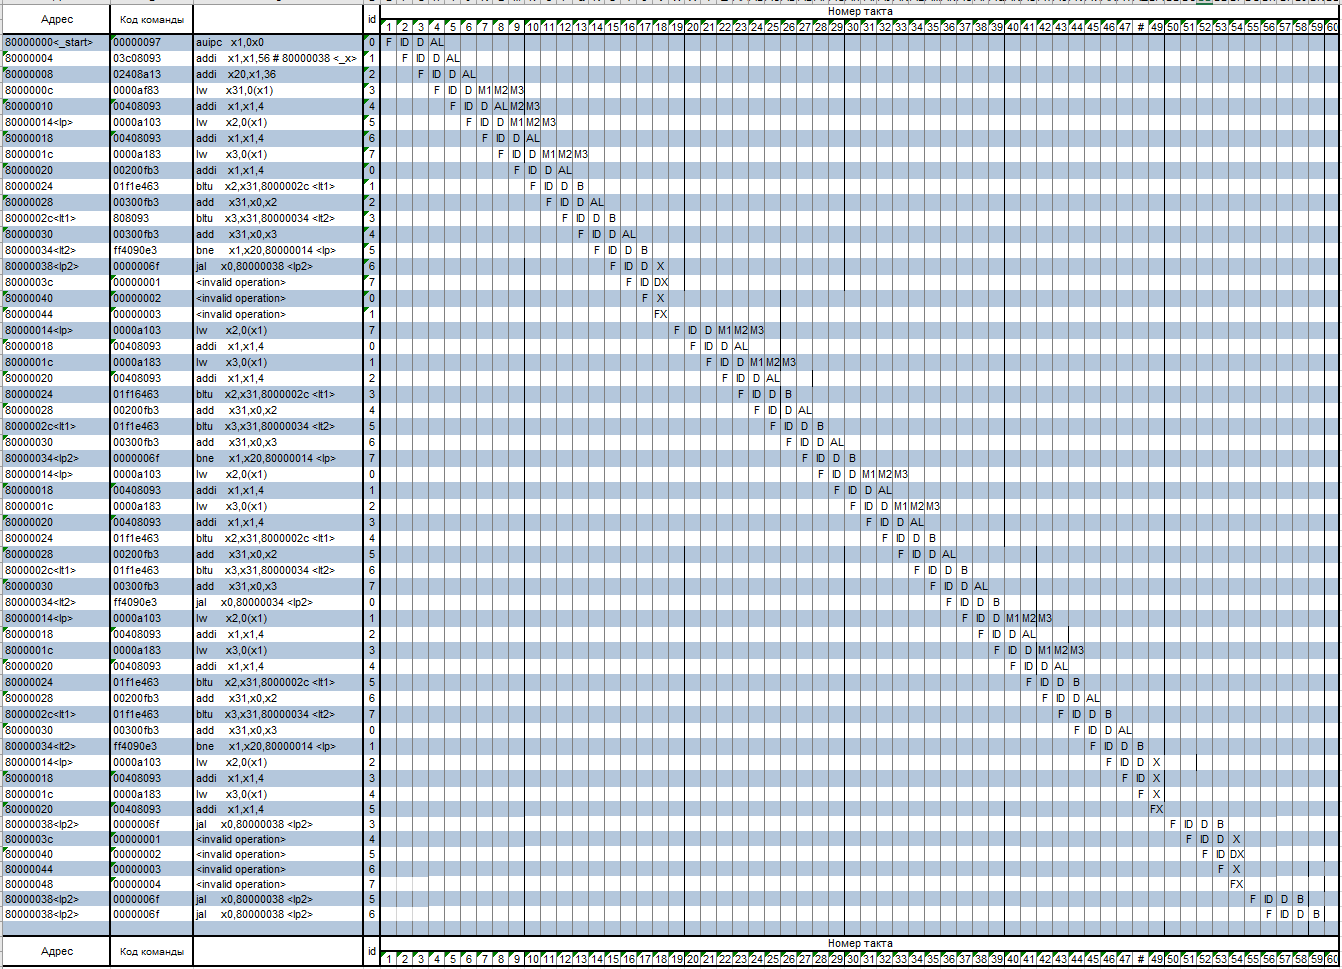
\includegraphics[width=170mm]{./img/trasa_opt.png}
    \caption{Трасса работы оптимизированной программы\label{overflow}}
\end{figure}
